\documentclass{IEEEtran}
\usepackage[english]{babel}
%\usepackage{subcaption}
%\usepackage{comment}
\usepackage{hyperref}
\usepackage{graphicx}
\usepackage{amsmath}
%\usepackage{authblk}
\graphicspath{{images/}}
\usepackage{geometry}
 \geometry{
 a4paper,
 total={170mm,257mm},
 left=15mm,
 top=15mm,
 }
\title{Path planning for Aerial Robots}
\author{
\begin{tabular}[t]{c@{\extracolsep{8em}}c} 
Eashwar Sathyamurthy  \hspace{2in} Akwasi A Obeng \\
Robotics Engineer \hspace{2in} Robotics Engineer \\ 
A. James Clark School of Engineering \hspace{1in} A. James Clark School of Engineering \\
University of Maryland \hspace{2in} University of Maryland \\
College Park, USA \hspace{2in} College Park, USA \\
eashwar@umd.edu \hspace{2in} obenga01@umd.edu
\end{tabular}
}

\begin{document}
\maketitle
\begin{abstract}
In recent times, the increase in the usage of automobiles has caused difficulty in transporting goods between two places.
As a result, the alternative use of employing aerial robots such as drones in transporting goods has gained a lot of popularity
due to reduced traffic and its ability to reach goal faster. However, aerial robots face the disadvantage of 
navigating obstacles such as avoiding collision with tall buildings, changing path to avoid dynamic obstacles etc. Due to these 
difficulties, path planning of drones becomes crucial. Hence, there is a need to develop a path planning algorithm which finds the shortest path to reach the goal whilst avoiding static and dynamic obstacles. In this report, we implemented sampling based path planning algorithms to enable the drone maneuver its environment in both static and dynamic environments.

\end{abstract}
\section{\textbf{Introduction}}
Drones in recent times are being used for surveillance in military and for transportation purposes. Recently, drones were used to transport kidneys. Hence, with the commercialization of drones, it is important to generate a path planning algorithm which can enable 
the drone to manuever its environment when faced with random obstacles. 
\begin{figure}[h]
    \centering
    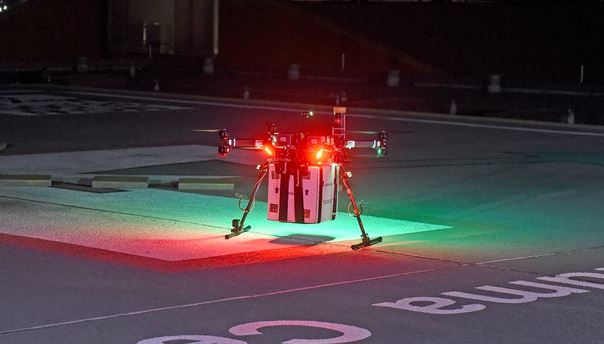
\includegraphics[width=7cm]{kidney}
    \caption{Drone delivering kidney}
    \label{fig:Drone delivering kidney}
\end{figure}
\newline
This report provides detailed implementation of RRT and RRT* sampling based algorithms both in 2D and 3D and provides comparison. Furthermore, the algorithm has been developed to avoid dynamic obstacles. This report provides the simulation results of both static and dynamic obstacle avoidance in 3D.
\section{\textbf{Plan of Action}}
\subsection{\textbf{Designing the environment}} 
The first step for visualing how well our code works is to generate a suitable environment that provides with it the ease of testing. 
The environment developed contains obstacles which should be avoided by the drone. The environment was designed both in 
3D and 2D (projection of 3D). Initially, we assume the environment to be static. Dynamic obstacles-that is, other drones- are added later in 3D environment to test our implementation.The figure below shows the environment in 2D as well as in 3D.
\begin{figure}[h]
    \centering
    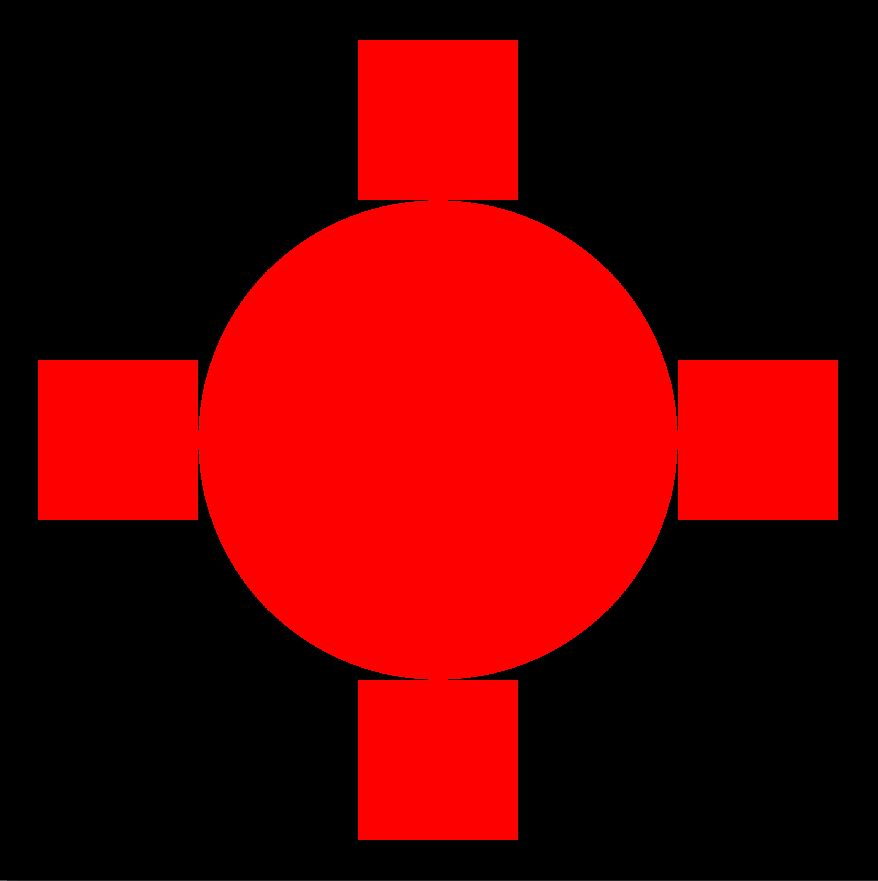
\includegraphics[width=6cm]{2dpygame}
    \caption{2D environment created using pygame}
    \label{fig:2D environment created using pygame}
\end{figure}
\begin{figure}[h]
    \centering
    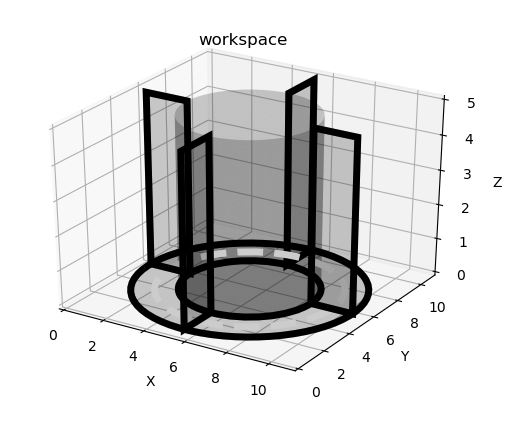
\includegraphics[width=9.5cm]{3dmatplotlib}
    \caption{3D environment created in matplotlib side view}
    \label{fig:3D environment created in matplotlib}
\end{figure}
\newline
Below is the equivalent environment created in ROS our implementation.
\newpage
\begin{figure}[h]
    \centering
    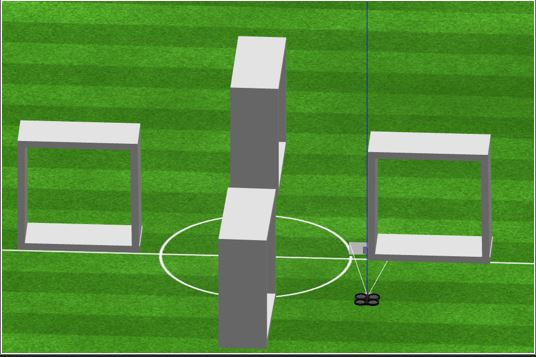
\includegraphics[width=8cm]{gazebo}
    \caption{3D environment created in matplotlib side view}
    \label{fig:3D environment created in matplotlib}
\end{figure}

\section{\textbf{Path planning method}} 
The path planning method choosen for the drone mainly depends on the type of obstacles present in the environment.
Below is a brief introduction to the types of obstacles as well as the different variants of RRT based methods used in the project.

\subsection{\textbf{Types of Obstacles}:}There are two types of obstacles. They are
\begin{enumerate}
\item \textbf{Static obstacles}: These obstacles do not move with respect to time. So, the obstacle space does not change with the passage of time. In an environment consisting of static obstacles, the generation of collision free optimal path happens only once.
\item \textbf{Dynamic obstacles}: These obstacles move with respect to time. So, the obstacle space constantly keep changing with the passage of time.  In an environment consisting of dynamic obstacles, the generation of  a  free optimal path may change continuously as dynamic obstacles can impede already generated path.
\end{enumerate} 

\subsection{\textbf{Sampling Based Algorithms}}
Below is a brief introduction to RRT with its variants.
\begin{enumerate}

\item \textbf{RRT (Rapidly Exploring Random Trees)}: In RRT, the map  is generated with the help of randomly sampled points. 
Newly, sampled points are joined to nearest nearest node of the RRT tree and this continues  until the target is reached. 
Each sampled point is checked against the robot workspace for validity. Refer to the pseudo code for detailed explanation of the 
algorithm.

\begin{figure}[h]
    \centering
    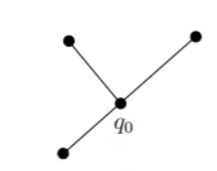
\includegraphics[width=3cm]{RRT1}
    \caption{RRT}
    \label{fig:RRT}
\end{figure}

\begin{figure}[h]
    \centering
    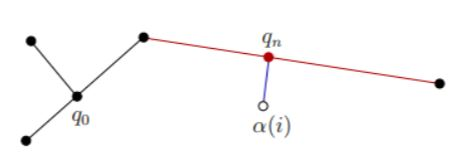
\includegraphics[width=6cm]{RRT2}
    \caption{Connecting the tree to nearest edge point}
    \label{fig:RRT}
\end{figure}
\begin{figure}[h]
    \centering
    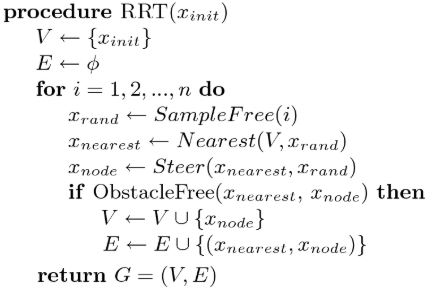
\includegraphics[width=8cm]{pRRT}
    \caption{RRT pseudo code}
    \label{fig:RRT}
\end{figure}
\item \textbf{RRT*}:
RRT* is just an extension of RRT but more computationally expensive. 
Compared to RRT, RRT* generates a more optimized path. 
The main difference between RRT and RRT* is that after joining a random node to a point, the nodes are \textbf{rewired} to improve the cost. \\ \\
In rewiring, all the nodes surrounding the newly added node are checked for better parent and this results in minimizing the 
cost-to-come. 
The rewiring process occurs around the neighborhood of the newly added node at some threholded distance. Thus,
 optimality of the path generated is achieved by finding path with minimum cost.
\\ \\ 
Although RRT* tries to find a more optimal path, the downside is that the rewiring occurs for all newly added nodes and this makes it 
a computationally expensive. The figure below shows the comparison of nodes exploration between RRT and RRT*. Refer below for the 
pseudo code for RRT*

\begin{figure}[h]
    \centering
    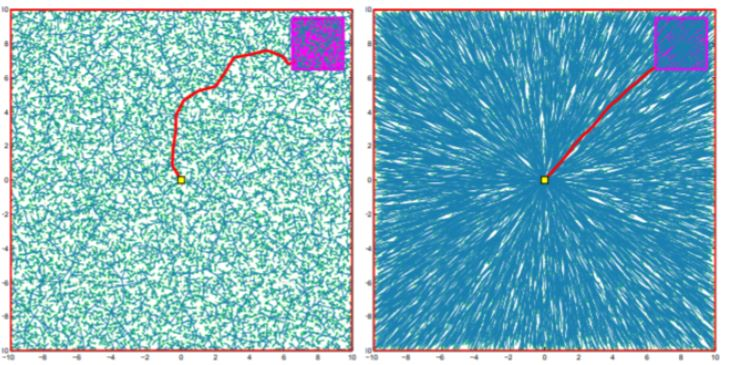
\includegraphics[width=8cm]{pRRT2}
    \caption{RRT  \hspace{1.8in}RRT*}
    \label{fig:RRT}
\end{figure}
The pseudo code for RRT* is given below.
\begin{figure}[h]
    \centering
    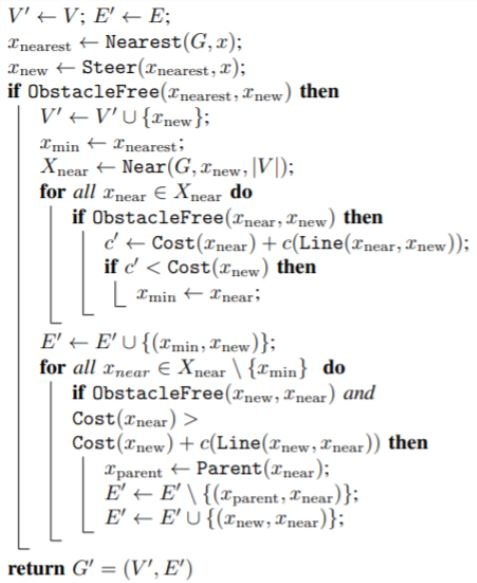
\includegraphics[width=8.5cm]{pRRT1}
    \caption{RRT* pseudo code}
    \label{fig:RRT}
\end{figure}
\\

\item {\textbf{Smoothing the Solution Path:}}
To avoid sharp edges in path generated, smoothing is carried out.
Ideally, smoothing should be carried out whilst planning.
However, only the solution path was smoothed in this problem due to the exhaustive workspace used. 
This however has the disadvantage of not being robust since the 
smoothed solution path might be in an obstacle workspace.
Gradient descent algorithm tries to minimize the error between the solution path and smoothened path.
The equation utilized in smooth is outlined below:

\boldmath	
\begin{equation}
y_i = y_i + \alpha(x_i - y_i) + \beta(y_{i+1} + y_{i-1} - 2*y_i)
\end{equation}
\unboldmath
\begin{center}
where $x_i$ is the $i^{th}$ solution coordinate \\
        $y_i$ is the  $i^{th}$ smoothened coordinate \\
	$y_{i-1}$ is the  $(i-1)^{th}$ smoothened coordinate \\
	$y_{i+1}$ is the  $(i+1)^{th}$ smoothened coordinate \\
	$\alpha$ is the smoothing coefficient which controls the degree of smoothing \\
	$\beta$ is the weight given to each solution node in the solution path \\
\end{center}
By tuning the $\alpha$ and $\beta$ parameters we can control the smoothing process.
\end{enumerate}
\section{ \textbf{Path planning for Dynamic obstacles:}}
For dynamic environment, other moving drones are used as dynamic obstacles.
The distance of the other drones are constantly tracked and should any of them 
obstruct the generated drone solution path
 and is close to the intended drone, replanning occurs.
 In replanning, the RRT/RRT* algorithm replans and finds a new path using current position of 
 the drone and the goal position with the updated environment(Obstacle blocking drone's path).
 Hence, the RRT/RRT* generates new path avoiding the obstacle. This process continues till the drone reaches the goal point. The pseudo code is given below[Reference 2]:
\begin{figure}[h]
    \centering
    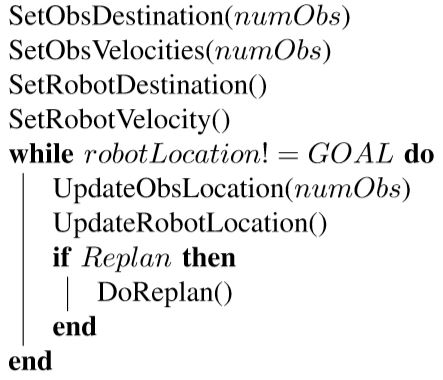
\includegraphics[width=6cm]{dynpseudocode}
    \caption{Dynamic Obstacle Avoidance using RRT pseudo code}
    \label{fig:Dynamic Obstacle Avoidance using RRT pseudo code}
\end{figure}
\section{\textbf{Software and Visualization tool Used}}
\begin{enumerate}
\item Python version 3
\item Matplotlib
\item Pygame
\end{enumerate}
\section{\textbf{Results}}
\subsection{\textbf{Implementation of RRT and RRT* in 2D environment}}
We first implemented RRT and RRT* in 2D using pygame. The following are the plots obtained:
\begin{figure}[h]
    \centering
    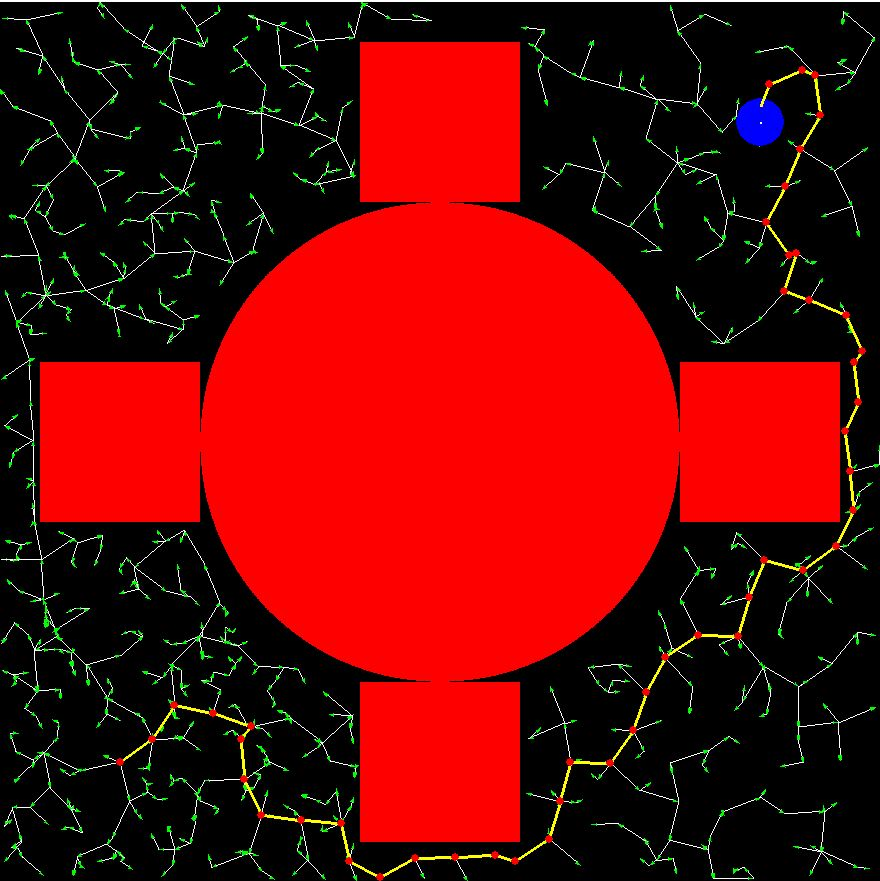
\includegraphics[width=7cm]{rrt2d}
    \caption{RRT implementation in 2D}
    \label{fig:RRT implementation in 2D}
\end{figure}
\newline 
The simulation time for RRT is about 2 seconds. We can clearly see that the path obtained is not optimal but the we get to the solution faster.
\newpage
\begin{figure}[h]
    \centering
    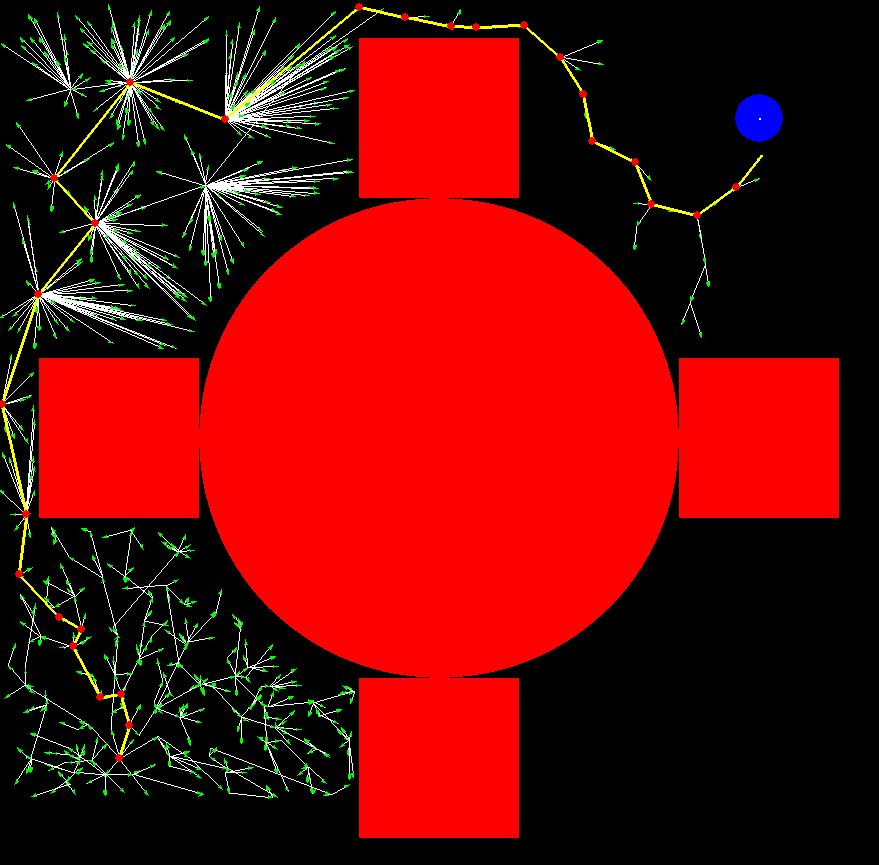
\includegraphics[width=7cm]{rrt2d1}
    \caption{RRT* implementation in 2D}
    \label{fig:RRT* implementation in 2D}
\end{figure} 
The simulation time for RRT* is about 113 seconds. We can clearly see that the path obtained is more optimized than RRT but the time taken to reach the solution is significantly increased. The nodes exploration is directed towards the goal position.

\subsection{\textbf{Implementation of RRT in 3D environment}}
As earlier mentioned, for simulation in 3D matplotlib package was used. The following are the results of RRT and RRT* for a static 3D environment.
\begin{figure}[h]
    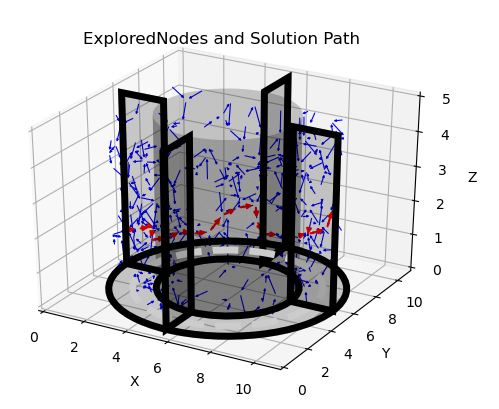
\includegraphics[width=7.5cm]{rrt3d}
    \caption{RRT implementation in 3D}
    \label{fig:RRT implementation in 3D}
\end{figure} 
\newpage
\begin{figure}[h]
    \centering
    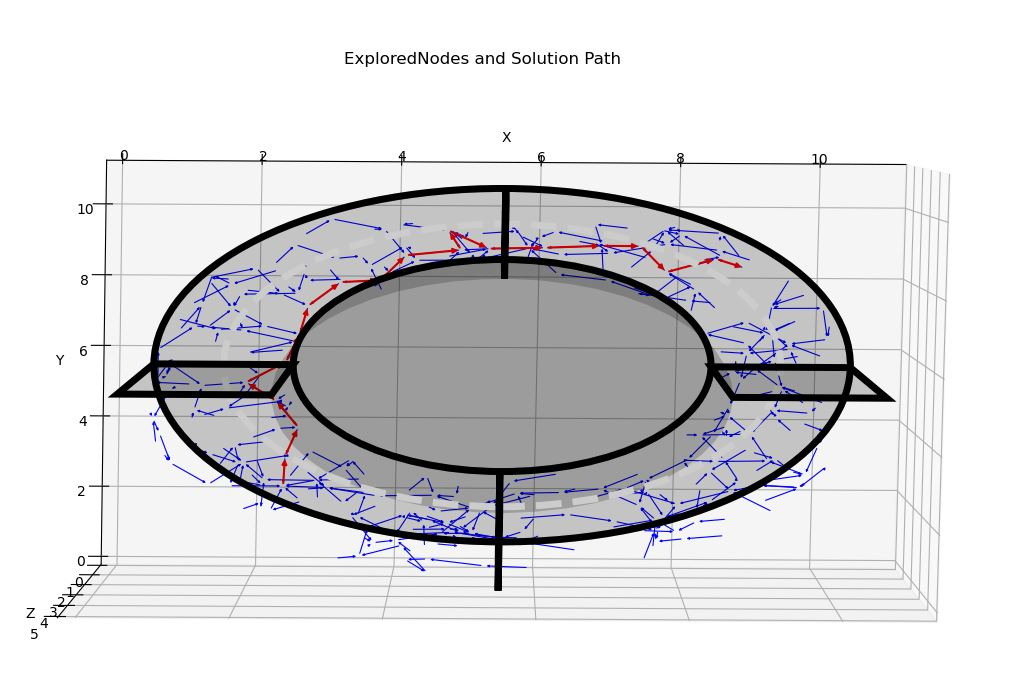
\includegraphics[width=10cm]{rrt3dtop}
    \caption{RRT implementation in 3D top view}
    \label{fig:RRT implementation in 3D top view}
\end{figure}
In addition to this, we have created an animation of drone using matplotlib which follows the solution trajectory.
 \begin{figure}[h]
    \centering
    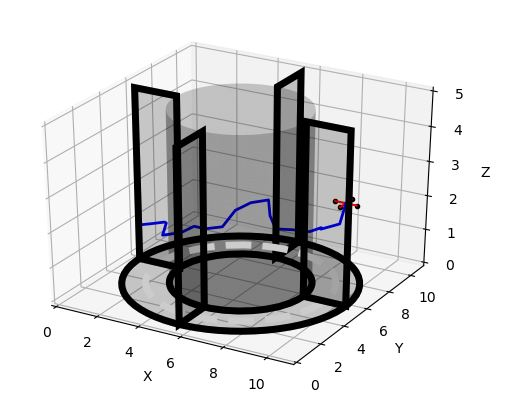
\includegraphics[width=9cm]{rrt3ddrone}
    \caption{RRT implementation drone animation}
    \label{fig:RRT implementation drone animation}
\end{figure}
\newline 
Currently, the path generated by RRT is not smoothened. By implementing the gradient descent algorithm, the solution path is smoothened. The following is the drone trajectory after the path of the drone is smoothened. As RRT generates new path each time, the path shown in the below figures may be little different from the above graphs but difference in the smoothness of the path is clearly seen.
\newpage
\begin{figure}[h]
    \centering
    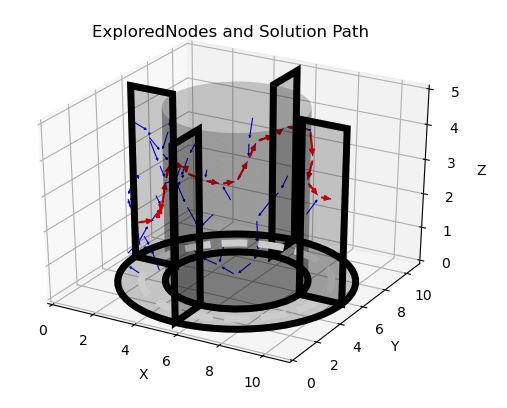
\includegraphics[width=7.5cm]{rrt3dsmooth}
    \caption{RRT implementation in 3D with smoothing}
    \label{fig:RRT implementation in 3D with smoothing}
\end{figure}

\begin{figure}[h]
    \centering
    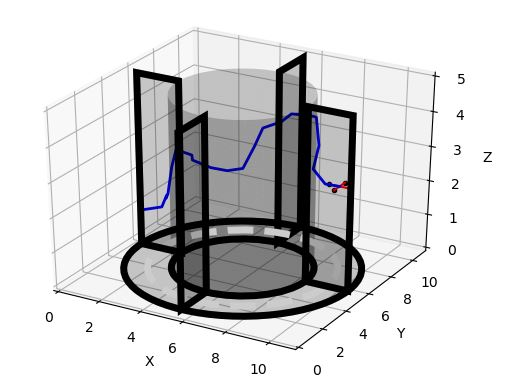
\includegraphics[width=7.5cm]{rrt3dsmoothdrone}
    \caption{RRT implementation in 3D smooth drone path}
    \label{fig:RRT implementation in 3D smooth drone path}
\end{figure}
\subsection{\textbf{Implementation of RRT* in 3D environment}}
Similar to RRT, we also implemented RRT* algorithm for a static 3D environment. Here are the results:
\begin{figure}[h]
    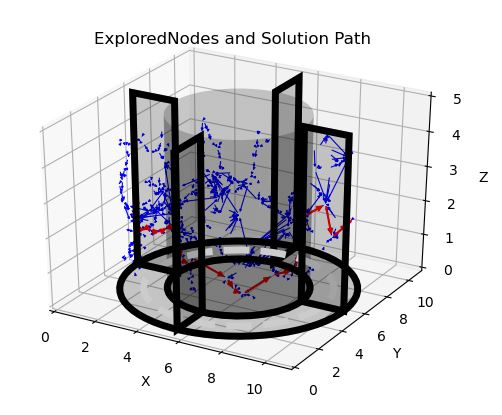
\includegraphics[width=7.5cm]{rrtstar3d}
    \caption{RRT* implementation in 3D}
    \label{fig:RRT* implementation in 3D}
\end{figure} 
\newpage
\begin{figure}[h]
    \centering
    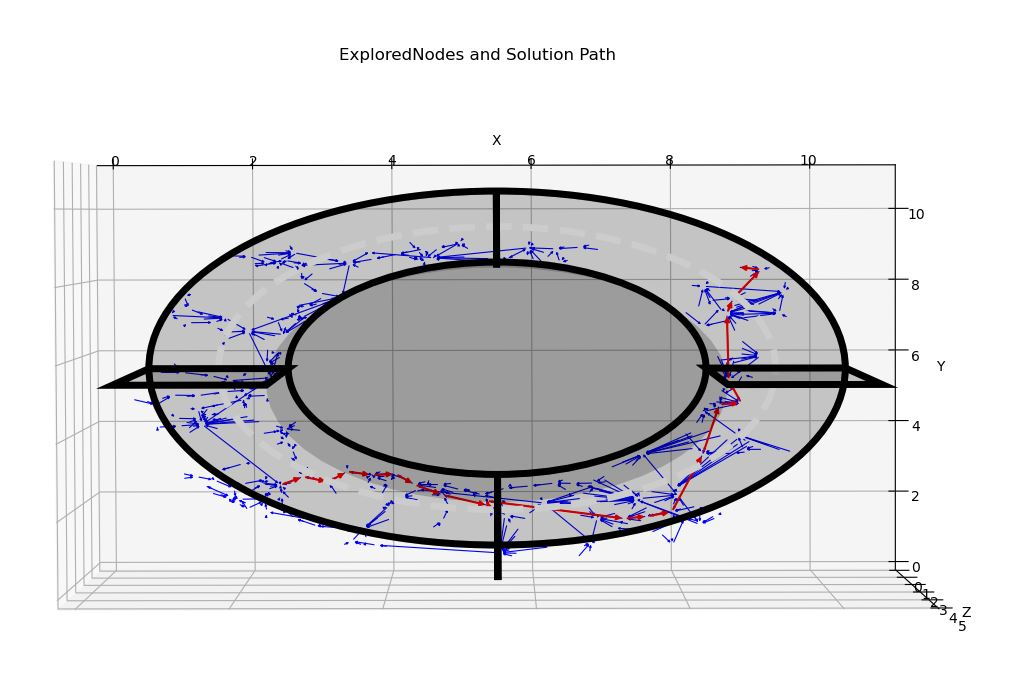
\includegraphics[width=9cm]{rrtstar3dtop}
    \caption{RRT* implementation in 3D top view}
    \label{fig:RRT* implementation in 3D top view}
\end{figure}
 \begin{figure}[h]
    \centering
    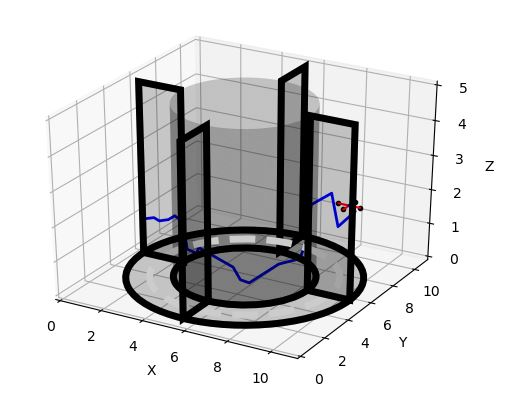
\includegraphics[width=8cm]{rrtstar3ddrone}
    \caption{RRT* implementation drone animation}
    \label{fig:RRT* implementation drone animation}
\end{figure}
After performing the smoothing, the following are the results:
\begin{figure}[h]
    \centering
    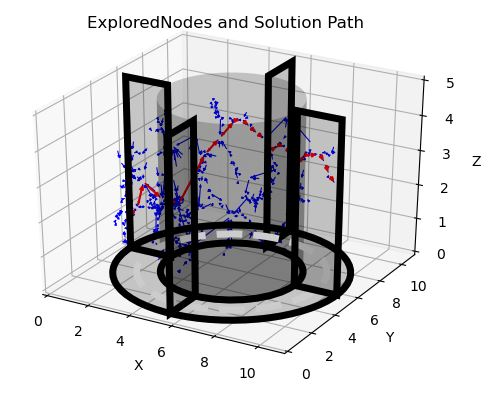
\includegraphics[width=7.5cm]{rrt3dstarsmooth}
    \caption{RRT* implementation in 3D with smoothing}
    \label{fig:RRT* implementation in 3D with smoothing}
\end{figure}
\begin{figure}[h]
    \centering
    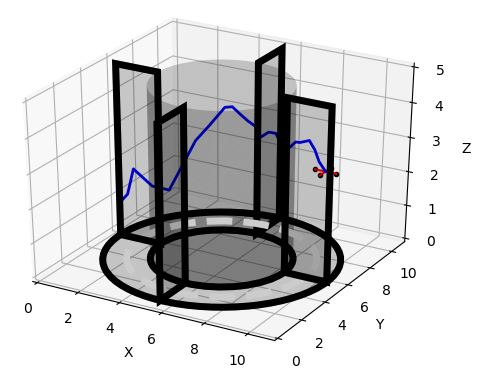
\includegraphics[width=7.5cm]{rrtstar3dsmoothdrone}
    \caption{RRT* implementation in 3D smooth drone path}
    \label{fig:RRT* implementation in 3D smooth drone path}
\end{figure}
\subsection{\textbf{Dynamic Environment path planning results:}}
We have developed RRT and RRT* algorithms to adapt to dynamic changes in the environment. Below sequence of images explains the pipeline with the output results. The following are the results obtained:
\begin{enumerate}
\item First RRT/RRT* generates the initial solution path considering the initial position of the obstacles(drones).
\begin{figure}[h]
    \centering
    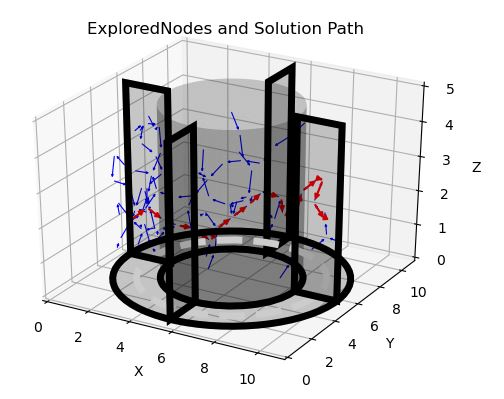
\includegraphics[width=8cm]{s2}
    \caption{Generating initial solution path}
    \label{fig:Generating initial solution path}
\end{figure}
\item The drone animation below shows the drone starting to the follow the initial generated solution path.
\begin{figure}[h]
    \centering
    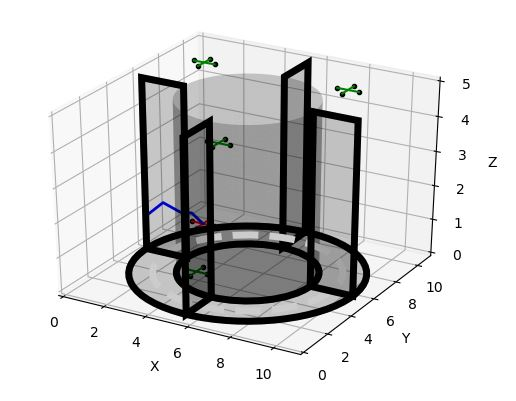
\includegraphics[width=8cm]{s1}
    \caption{Drone following the initial solution path}
    \label{fig:Drone following the initial solution path}
\end{figure}
\item In the above picture, one of the obstacle drone was obstructing as well as close to the drone. Hence, replanning of the path occurs.
\begin{figure}[h]
    \centering
    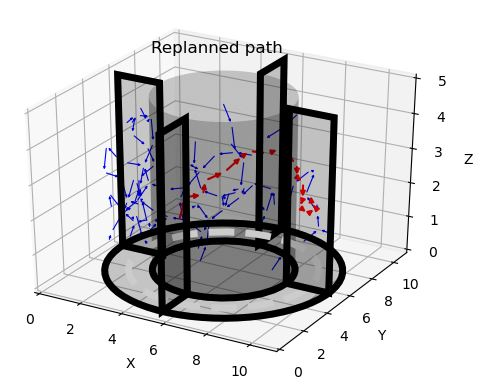
\includegraphics[width=8cm]{replanned}
    \caption{Replanning of drone path from current position}
    \label{fig:Replanning of drone path from current position}
\end{figure}
\item Now the figure below shows the animation of the drone following the replanned path
\begin{figure}[h]
    \centering
    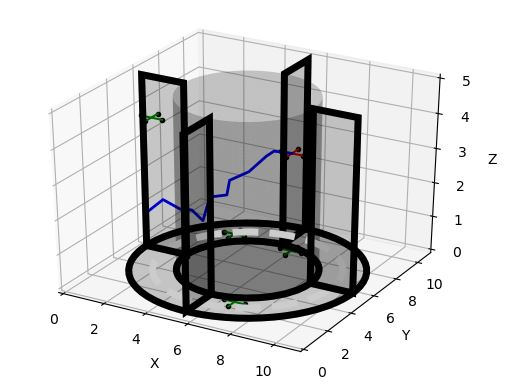
\includegraphics[width=8cm]{replanned1}
    \caption{Drone following replanned path}
    \label{fig:Drone following replanned path}
\end{figure}
\end{enumerate}
\section{\textbf{Goal Achieved:}}
\begin{enumerate}
\item Successfully implemented RRT and RRT* algorithms in 2D in static environment.
\item Successfully created a dynamic obstacle space in 3D.
\item Successfully implemented RRT and RRT* algorithms in static and dynamic environment in 3D.
\item Successfully smoothened the solution path using gradient descent algorithm.
\end{enumerate}
\section{\textbf{Future Scope}}
Our future goal would be to integrate the algorithm with ROS and provide a simulation in gazebo. 
\section{References:}
\begin{enumerate}
\item The modified quadrotor.py was initially coded by Daniel-S-Ingram, Refer,
https://github.com/daniel-s-ingram
\item \href{https://arxiv.org/pdf/1704.04585.pdf}{\underline{Dynamic Obstacle Avoidance pseudo code}}
\end{enumerate}
\end{document}

